


\subsubsection{KW42 + KW43:}
\begin{quote}
	\subsubsection*{Arbeit in der Schule}
	
	Im Unity Asset Store wurde der Character Pack: Free Sample
	heruntergeladen und in das Projekt eingefügt. Anschließend wurde der
	Prefab Model in die Scene eingefügt. In der Scene wurde auch mit einem
	3D-Cube der Boden erstellt. Danach wurde der Animator
	Controller und das Character Movement Programm, dem Charakter
	zugewiesen.
	
	Ergebnis: Der Charakter kann grundlegende Bewegungen wie Renen, Drehen
	und Springen ohne Probleme ausführen.
	\begin{figure}
		\centering
		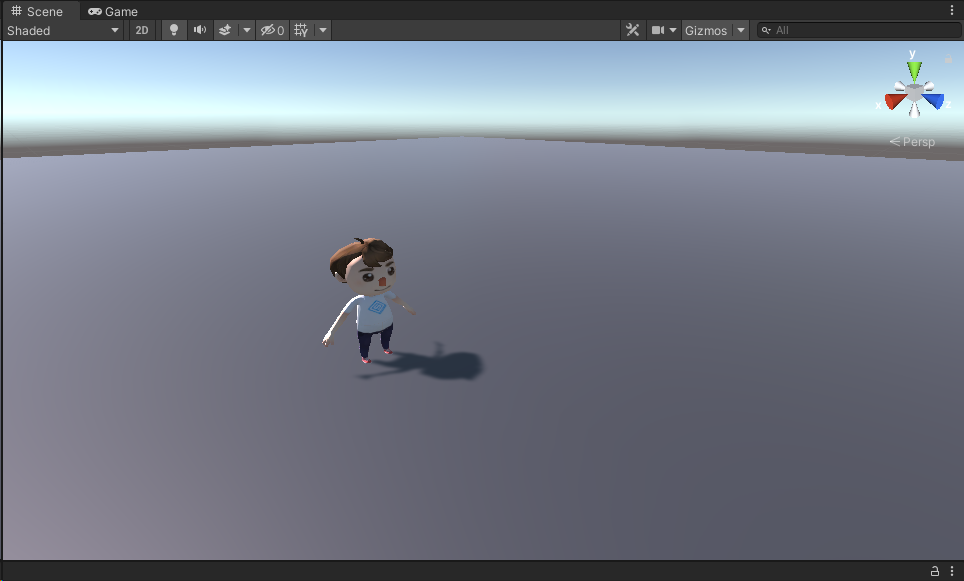
\includegraphics[width=0.6\linewidth]{img/SemihSoenmez_IMG/Main-Charakter_SS_KW45_131121}
		\caption{}
		\label{fig:main-charaktersskw45131121}
	\end{figure}
	
	
	Anschließend habe ich ein bisschen rechechiert wie ich die Gegner
	programmieren soll, da dies meine nächste Aufgabe ist.

	\subsubsection*{Arbeit außerhalb der Schule}
	Meine nächste Aufgabe ist es die Gegner zu programmieren. Dafür habe ich
	auf der Seite \url{www.mixamo.com} ein Lehrer-Charakter und eine
	Lauf-Animation heruntergeladen und sie im Projekt eingefügt.
	
	Links:


	Youtube-tutorial für Charakter: \footcite{CharakterTutorial}
	
	Walking Animation: \footcite{WalkingAnimation}
	
	Charakter Leonard: \footcite{LehrerCharakter}
	
	Der eingefügte Charakter war in der Scene grau zu sehen. Also habe ich
	sein Material vom Charakter im Inspector window extrahiert. Anschließend
	war der Charakter wieder bunt zu sehen.

	\begin{figure}
		\centering
		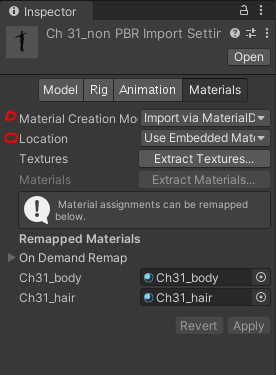
\includegraphics[width=0.3\linewidth]{../../mazerun/dokumentation/img/SemihSoenmez_IMG/Inspector_SS_KW44_251021}
		\caption{}
		\label{fig:inspectorsskw44251021}
	\end{figure}

	
	Jetzt muss dem Charakter die Walkinganimation zugewiesen werden.
	
	Inspector window: Rig:
	
	\begin{itemize}
		\item
		Animation Type auf "Humanoid"" und Avatar Definiton auf "Copy from
		other Avatar" umgestellt
		\item
		Beim Source den teacher Avatar ausgewählt
	\end{itemize}
	
	Danach wurde ein Animator Controller erstellt, in der wir unsere
	Animation eingefügt haben. Wie im Bild zusehen ist, wird beim Starten
	des Spiels, der Start Walking Animation durchgeführt.
	\begin{center}
		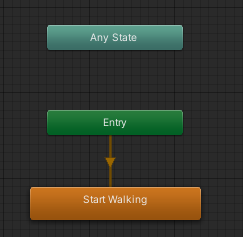
\includegraphics[frame, height=6cm]{img/SemihSoenmez_IMG/StateMachine_SS_KW44_251021.png}
	\end{center}
\end{quote}

